\chapter{Overview of the approach}
\label{chap:overview}

This case study concentrates on the connection between the design time, and the runtime domain. Our goal is to connect these two domains, and make a solution that generally can support the relation between the design, and runtime.

\begin{figure}[h]
	\centering
	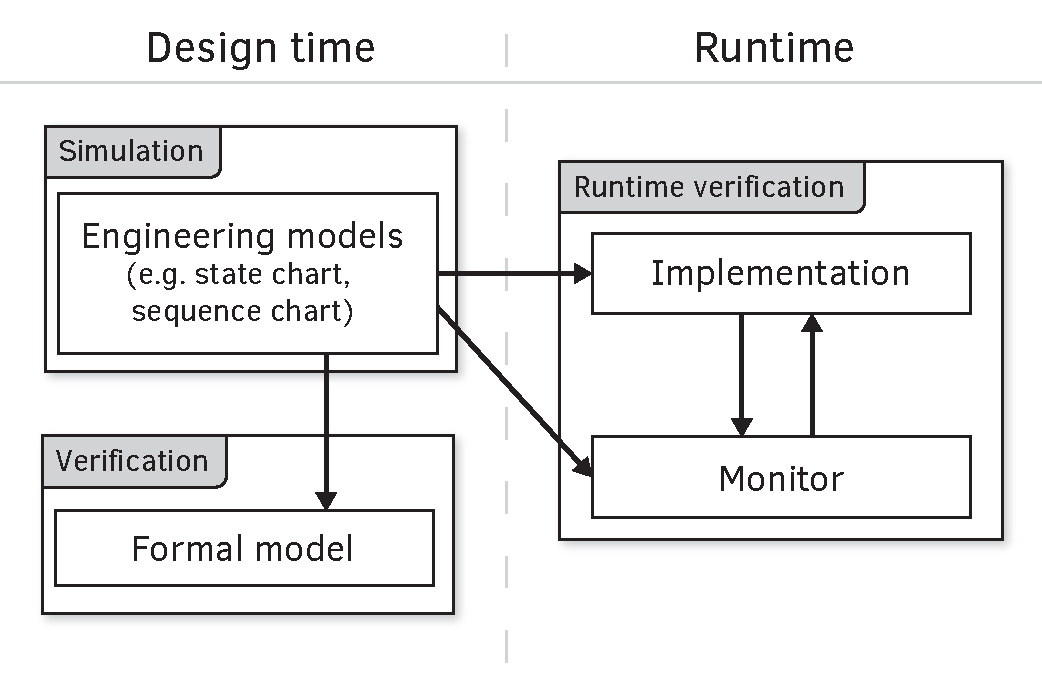
\includegraphics[width=0.75\linewidth]{include/figures/chapter_3/abstract_overview}
	\caption{Connection between runtime and design time elements}
	\label{fig:overview:abstract_overview}
\end{figure}

Solutions which connect two, or three elements of \cref{fig:overview:abstract_overview} are existing, but there is no tool which integrate all these in one tool with interchangeable formalisms.
\\[1ex]

\noindent Let us consider the following example:

We want to design a system, where we have a model of our system, described by using a formalism (e.g. state chart, sequence chart), and we want to:
\begin{itemize}
	\item Generate the implementation from the model.
	\item Implement runtime verification into our implementation, by monitoring the application.
	\item We have multiple monitoring systems, and if a components verification state changes we want to react.
\end{itemize}